% =====================================================================
% RL Final Project Report
% Compile on Overleaf with pdfLaTeX.  All required images are in ./figures/.
% =====================================================================
\documentclass[twocolumn,a4paper,10pt]{article}

\usepackage[a4paper,top=18mm,bottom=20mm,left=15mm,right=15mm,columnsep=6mm]{geometry}
\usepackage[T1]{fontenc}
\usepackage[utf8]{inputenc}
\usepackage{lmodern}
\usepackage{microtype}
\usepackage{graphicx}
\usepackage{booktabs}
\usepackage{array}
\usepackage{caption}
\usepackage{subcaption}
\usepackage{xcolor}
\usepackage{amsmath,amssymb}
\usepackage{enumitem}
\usepackage{hyperref}
\usepackage{tikz}
\usepackage{tcolorbox}
\usepackage{listings}
\tcbuselibrary{listings,skins,breakable}
\usetikzlibrary{positioning,arrows.meta,shadows,fit,calc}

\hypersetup{
  colorlinks=true,
  linkcolor=blue!55!black,
  citecolor=blue!55!black,
  urlcolor=blue!55!black
}

\setlength{\parindent}{0pt}
\setlength{\parskip}{2.2pt}
\setlist{nosep,leftmargin=*}
\captionsetup{font=small,labelfont=bf,skip=3pt}
\renewcommand{\arraystretch}{1.08}

\definecolor{cBlue}{HTML}{1F77B4}
\definecolor{cOrange}{HTML}{FF7F0E}
\definecolor{cGreen}{HTML}{2CA02C}
\definecolor{cRed}{HTML}{D62728}
\definecolor{cTeal}{HTML}{17BECF}
\definecolor{cGray}{HTML}{6C757D}
\definecolor{boxBg}{HTML}{F5F7FA}

\newcommand{\headcell}[1]{\textbf{#1}}
\newcommand{\repo}{\href{https://github.com/vishal36-pop/project}{https://github.com/vishal36-pop/project}}
\newcommand{\demolink}{\href{https://iiitbac-my.sharepoint.com/:f:/g/personal/vishal_sriram_iiitb_ac_in/IgD556iWK6AsR59jMQwmS-3IARv652K0kij4iknw9YbVtEg?e=tKtRGe}{Demo video (MP4)}}

% =====================================================================
\title{\vspace{-1.2em}
       \Large\textbf{Vision-Based Continuous Drone Navigation\\
       in Wind Environments using PPO with a Vision Transformer}\vspace{-0.4em}}

\author{%
  \normalsize
  \begin{tabular}{c}
  Vishal Reddy K (BT2024102) \quad
  Harsha Vardhan (BT2024106)\\
  Vishal Sriram (BT2024036) \quad
  Lohith Pasumarthi (BT2024248)\\[-1pt]
  \footnotesize International Institute of Information Technology, Bangalore\\
  \footnotesize Reinforcement Learning -- Final Course Project
  \end{tabular}
}
\date{}

\begin{document}
\twocolumn[{%
  \maketitle
  \vspace{-2.3em}
  \begin{center}
  \begin{minipage}{0.94\textwidth}
  \small
  \noindent\textbf{Abstract.}
  We study indoor drone navigation as a real-world reinforcement learning
  problem: a quadrotor must reach a goal through a cluttered corridor while
  resisting wind and avoiding collisions.  The task has continuous controls,
  partial observability from a front camera, delayed consequences, and
  safety-critical failures, making it a natural fit for RL.  We formulate the
  problem as an MDP/POMDP and train a multimodal \textbf{PPO} actor-critic
  with a \textbf{Vision Transformer (ViT)} image encoder fused with low-level
  state features.  The final system is evaluated against \textbf{DDPG} and
  \textbf{SAC} baselines and six controlled ablations covering reward scale,
  curriculum learning, advantage normalization, image vs. state observations,
  ViT vs. CNN encoders, and domain randomization.  On the final-stage
  evaluation ($N=30$), PPO+ViT reaches \textbf{100\% success} with
  \textbf{0\% collision}; DDPG/SAC fail under the same cluttered windy setting.
  A generalization suite shows robustness to wind, clutter, turns, narrow
  corridors, and sensor noise, with a clear limitation on longer corridor
  geometry.
  \end{minipage}
  \end{center}
  \vspace{1.1em}
}]

% =====================================================================
\section{Introduction}

Autonomous drones are useful for inspection, search-and-rescue, inventory
monitoring, and indoor delivery.  These settings require flight through
constrained spaces where GPS is unavailable, obstacles can move, and airflow
disturbances can push the vehicle away from safe trajectories.  Classical
planning and control pipelines usually require explicit maps, reliable
localization, and manually tuned controllers; however, visual navigation from
raw images is partially observable and highly coupled with control.

\textbf{Why reinforcement learning?}
RL directly optimizes sequential decision making: the drone can learn how
short-term velocity choices affect future collision risk and goal progress.
Continuous-control RL is especially appropriate because the action is not a
discrete left/right command but a velocity vector $(v_x,v_y,v_z)$.  We choose
PPO as the primary algorithm because clipped on-policy updates are stable in
high-dimensional policy spaces \cite{schulman2017ppo}, while off-policy
actor-critic baselines (DDPG/SAC) provide meaningful comparisons for
continuous control \cite{lillicrap2015ddpg,haarnoja2018sac}.

\textbf{Contributions.}
\begin{itemize}
  \item A PyBullet drone-corridor environment with RGB observations, state
  features, continuous velocity control, moving obstacles, sensor noise, and
  Ornstein--Uhlenbeck (OU) wind.
  \item A PPO+ViT multimodal actor-critic trained with a six-stage curriculum.
  \item A detailed reward design and ablation analysis explaining what each
  experimental change tests and how it affects learning.
  \item Quantitative comparisons, generalization tests, and a linked demo
  video for qualitative inspection.
\end{itemize}

% =====================================================================
\section{Related Work / Literature Survey}

\textbf{Continuous control RL.}
DDPG learns a deterministic continuous policy using an actor, critic, target
networks, and replay buffer \cite{lillicrap2015ddpg}.  It is sample efficient
in some low-dimensional tasks, but can become unstable when critic errors are
amplified through the actor.  SAC improves off-policy control by maximizing
both reward and entropy, which encourages exploration and robust stochastic
policies \cite{haarnoja2018sac}.  PPO uses a clipped surrogate objective to
limit destructive policy updates, trading sample efficiency for reliable
optimization \cite{schulman2017ppo}.  This stability is valuable when the
policy includes a vision encoder.

\textbf{Vision-based RL and transformers.}
CNNs are common image encoders in RL, but Vision Transformers split the image
into patches and use self-attention to model long-range spatial relationships
\cite{dosovitskiy2020vit}.  In corridor navigation, such global context can
help distinguish open passage structure from nearby clutter.  We compare ViT
against a CNN encoder and a state-only policy to test whether vision and the
encoder choice matter.

\textbf{Curriculum learning.}
Curriculum learning trains agents on progressively harder versions of a task
\cite{bengio2009curriculum}.  For drone navigation, beginning with wide
obstacle-free corridors reduces early collision-dominated rollouts; later
stages introduce clutter, moving obstacles, wind, and noise.  This mirrors
real robotics practice: learn coarse navigation first, then stress-test
robustness.

% =====================================================================
\section{Problem Formulation}

We formulate the environment as a finite-horizon Markov Decision Process with
partial observability from camera images:
\[
  \mathcal{M}=(\mathcal{S},\mathcal{A},P,R,\gamma,\rho_0,T).
\]

\textbf{State space.}
The true simulator state includes drone pose and velocity, obstacle poses,
wall geometry, wind state, and the goal.  The agent observes
$o_t=[I_t,s_t]$, where $I_t\in\mathbb{R}^{64\times64\times3}$ is the
front-facing RGB image and $s_t\in\mathbb{R}^{15}$ contains four wall
distances, forward clearance, velocity, yaw error, goal direction, and the
previous action.  This makes the task a POMDP in practice.

\textbf{Action space.}
The action is continuous:
\[
  a_t=(v_x,v_y,v_z)\in[-1,1]^3,
\]
which is scaled internally to $\pm 3.0$ m/s and tracked by a velocity-PD
controller.

\textbf{Transition dynamics.}
PyBullet simulates rigid-body dynamics at 240 Hz; the policy acts at 30 Hz.
OU wind is applied as an external force, producing temporally correlated
disturbances:
\[
  dx_t=-\theta x_t\,dt + \sigma\,dW_t.
\]
The transition also includes collision contacts, moving obstacles, sensor
noise, and randomized corridor layouts from the environment seed.

\textbf{Episode termination.}
Episodes terminate when the drone reaches the goal radius, collides with an
obstacle/wall/floor, leaves valid bounds, or reaches the maximum step budget
(1500 control steps).

\begin{figure}[!t]
\centering
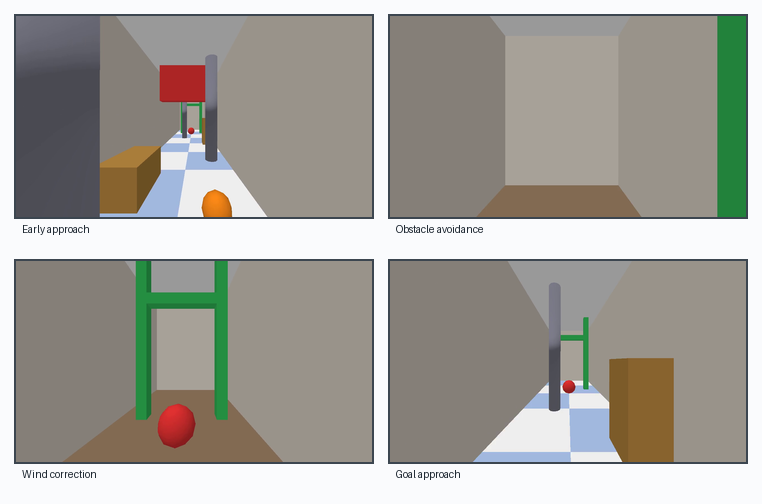
\includegraphics[width=\linewidth]{figures/fig_demo_montage.png}
\caption{Representative frames from the 720p demo video.  The policy uses
64$\times$64 observations internally; the figure is rendered at higher
resolution only for visualization.}
\label{fig:envsnap}
\end{figure}

% =====================================================================
\section{Methodology}

\subsection{Environment and Curriculum}

The final training environment contains a 10 m corridor, static and moving
obstacles, wind, and noisy sensors.  To avoid early training being dominated
by immediate collisions, we use the curriculum in Table~\ref{tab:curriculum}.
The stages isolate different sources of difficulty: corridor narrowing tests
lateral control; obstacle density tests perception and avoidance; moving
obstacles test reactive control; wind and noise test robustness.

\begin{table}[!t]
\centering
\caption{Curriculum stages used for PPO+ViT training.}
\label{tab:curriculum}
\resizebox{\linewidth}{!}{%
\begin{tabular}{@{}lccccc@{}}
\toprule
\headcell{Stage} & \headcell{Width} & \headcell{Obs. dens.} &
\headcell{Moving} & \headcell{Wind $\sigma$} & \headcell{Noise}\\
\midrule
1. wide straight      & 3.0 & 0.0 & no  & 0.00 & 0.00\\
2. narrow corridor    & 2.6 & 0.0 & no  & 0.00 & 0.00\\
3. with obstacles     & 2.5 & 0.7 & no  & 0.00 & 0.00\\
4. moving obstacles   & 2.5 & 1.0 & yes & 0.00 & 0.00\\
5. wind introduction  & 2.0 & 1.0 & yes & 0.25 & 0.05\\
6. full wind          & 2.0 & 1.0 & yes & 0.50 & 0.05\\
\bottomrule
\end{tabular}}
\end{table}

\subsection{PPO+ViT Architecture}

The policy is a Gaussian actor-critic.  The image branch is a ViT with
patch size 8, embedding dimension 128, depth 4, and 4 attention heads,
producing a 192-dimensional visual feature.  The state branch is an MLP
mapping $15\to128$.  The fused 320-dimensional representation is passed
through a $256\to256$ shared trunk and split into an actor head
$(\mu,\log\sigma)$ and critic head $V(s)$.

\begin{figure*}[!t]
\centering
\resizebox{0.93\textwidth}{!}{%
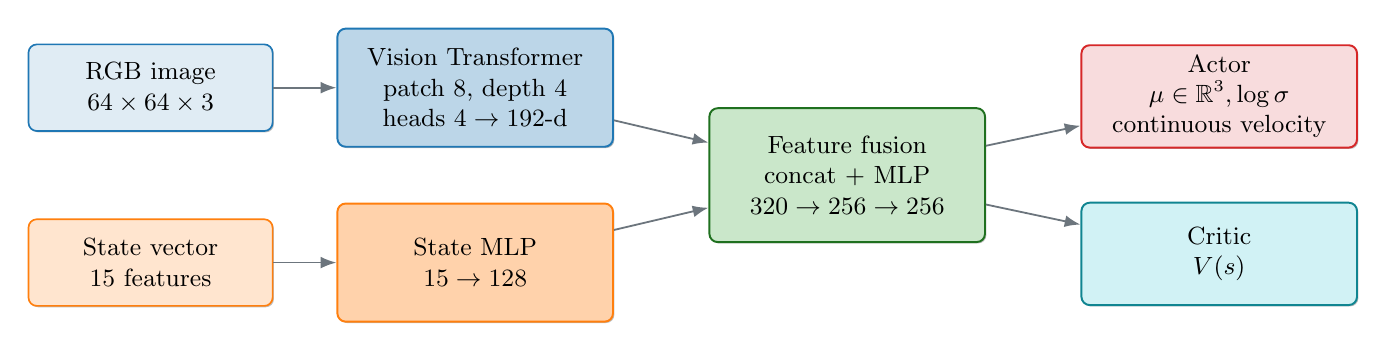
\begin{tikzpicture}[
  node distance=6mm and 8mm,
  every node/.style={font=\small, align=center, rounded corners=3pt,
    drop shadow={shadow xshift=0.5pt, shadow yshift=-0.5pt}},
  input/.style={fill=cBlue!14, draw=cBlue, line width=0.6pt,
    minimum width=31mm, minimum height=11mm},
  state/.style={fill=cOrange!20, draw=cOrange, line width=0.6pt,
    minimum width=31mm, minimum height=11mm},
  enc/.style={fill=cBlue!30, draw=cBlue, line width=0.7pt,
    minimum width=35mm, minimum height=15mm},
  mlp/.style={fill=cOrange!35, draw=cOrange, line width=0.7pt,
    minimum width=35mm, minimum height=15mm},
  fuse/.style={fill=cGreen!25, draw=cGreen!70!black, line width=0.7pt,
    minimum width=35mm, minimum height=17mm},
  actor/.style={fill=cRed!16, draw=cRed, line width=0.7pt,
    minimum width=35mm, minimum height=13mm},
  critic/.style={fill=cTeal!20, draw=cTeal!70!black, line width=0.7pt,
    minimum width=35mm, minimum height=13mm},
  arr/.style={-{Latex[length=2mm]}, line width=0.65pt, color=cGray}]

  \node[input] (img) {RGB image\\$64\times64\times3$};
  \node[state, below=11mm of img] (slow) {State vector\\15 features};

  \node[enc, right=of img] (vit) {Vision Transformer\\patch $8$, depth $4$\\heads $4\to192$-d};
  \node[mlp, right=of slow] (senc) {State MLP\\$15\to128$};

  \coordinate (mid) at ($(vit.east)!0.5!(senc.east)$);
  \node[fuse, anchor=west] (fusion) at ($(mid)+(12mm,0)$)
    {Feature fusion\\concat $+$ MLP\\$320\to256\to256$};

  \node[actor, anchor=west] (actor) at ($(fusion.east)+(12mm,10mm)$)
    {Actor\\$\mu\in\mathbb{R}^3,\log\sigma$\\continuous velocity};
  \node[critic, anchor=west] (critic) at ($(fusion.east)+(12mm,-10mm)$)
    {Critic\\$V(s)$};

  \draw[arr] (img) -- (vit);
  \draw[arr] (slow) -- (senc);
  \draw[arr] (vit) -- (fusion);
  \draw[arr] (senc) -- (fusion);
  \draw[arr] (fusion) -- (actor);
  \draw[arr] (fusion) -- (critic);
\end{tikzpicture}}
\caption{Multimodal PPO actor-critic.  The ViT provides global visual
context while the low-dimensional state branch supplies geometric and
control signals.  The same fused representation supports both the policy and
value estimate.}
\label{fig:architecture}
\end{figure*}

\subsection{Training Pipeline and Hyperparameters}

The PPO rollout uses 4 vectorized environments, 2048 steps per rollout,
10 epochs, batch size 512, discount $\gamma=0.99$, GAE $\lambda=0.95$,
clip range 0.2, entropy coefficient 0.01, value coefficient 0.5, gradient
norm clipping at 0.5, and a linear learning-rate schedule from $10^{-4}$ to
$10^{-5}$.  Mixed precision is enabled on GPU.  Advantage normalization and
clipped value loss are used to reduce update variance.

PPO+ViT was chosen as the primary method because the environment combines
vision, continuous control, sparse catastrophic failures, and nonstationary
curriculum stages.  PPO is less sample efficient than replay-based methods
but is more stable when the policy contains a deep visual encoder.  DDPG and
SAC were retained as baselines to test whether off-policy continuous-control
methods can solve the same task with low-dimensional state observations.

% =====================================================================
\section{Reward Design}

The reward was designed to balance three competing goals: move toward the
goal, avoid unsafe behavior, and prevent degenerate policies that survive
without completing the corridor.  The implemented report reward is
\[
R_t=r_{\text{distance}}+r_{\text{goal}}+r_{\text{time}}
    +r_{\text{timeout}}+r_{\text{collision}} .
\]
The distance term is normalized by the initial goal distance, so progress is
comparable across layouts.  Wind is not rewarded directly; instead, wind is
introduced through transition dynamics.  A good policy receives high reward
only if it maintains progress despite wind disturbances.  This avoids
rewarding wind-specific artifacts and encourages robust closed-loop control.

\begin{table*}[!t]
\centering
\caption{Reward components and intended behavior.  Values are from the final
report configuration.}
\label{tab:reward}
\resizebox{0.94\textwidth}{!}{%
\begin{tabular}{@{}llll@{}}
\toprule
\headcell{Event / component} & \headcell{Reward value} &
\headcell{Purpose} & \headcell{Learning effect}\\
\midrule
Forward distance progress &
$100\,\Delta d/d_0$ &
Encourage movement toward the goal &
Provides dense gradient before the sparse goal signal.\\
Goal reached &
$+30$ &
Terminate successful episodes with high return &
Separates true completion from merely surviving.\\
Collision &
$-50$ &
Strongly discourage hitting walls/obstacles/floor &
Makes unsafe exploration clearly suboptimal.\\
Timeout &
$-20$ &
Discourage hovering or slow indecisive policies &
Pushes the agent to finish within the horizon.\\
Per-step time cost &
$-0.002$ &
Mild efficiency pressure &
Breaks ties in favor of shorter, smoother paths.\\
Wind disturbance &
implicit in $P(s_{t+1}|s_t,a_t)$ &
Require robust correction under external force &
Rewards policies that keep progress under perturbation.\\
\bottomrule
\end{tabular}}
\end{table*}

Reward shaping substantially improved stability: without dense progress,
most early trajectories end in collision before observing a useful success
signal.  However, the reward-scale ablation shows that scaling matters.
Reducing the distance scale from 100 to 1 still permits success, but the
policy takes much longer episodes and receives much lower return, indicating
that the dense term mainly accelerates learning and improves efficiency.

% =====================================================================
\section{Experiments and Ablation Studies}

All evaluations use the latest checkpoint for each run and evaluate in the
final curriculum stage with $N=30$ episodes.  We ran experiments to answer
four questions: (i) which RL algorithm is most stable, (ii) whether visual
input is necessary, (iii) whether the ViT matters compared with CNN features,
and (iv) how curriculum, reward scaling, and domain randomization affect the
trained behavior.

\subsection{Algorithms Compared}

\textbf{PPO+ViT.}
Main method.  It combines clipped on-policy updates with a multimodal visual
policy.  It is expected to be stable but less sample efficient.

\textbf{DDPG.}
Chosen because the proposal required a Q-learning-family continuous-control
baseline.  It uses deterministic policy gradients and a replay buffer, which
can be sample efficient but is sensitive to critic over-estimation.

\textbf{SAC.}
Chosen as a stronger off-policy baseline.  Entropy maximization should help
exploration, but the method still depends on accurate value estimates.

\subsection{Controlled Ablations}

\begin{table*}[!t]
\centering
\caption{Ablation study summary.  Each experiment changes one design choice
relative to PPO+ViT unless stated otherwise.}
\label{tab:ablation}
\resizebox{0.96\textwidth}{!}{%
\begin{tabular}{@{}p{0.20\textwidth}p{0.28\textwidth}p{0.35\textwidth}rrr@{}}
\toprule
\headcell{Experiment} & \headcell{Change} & \headcell{Interpretation} &
\headcell{Succ.} & \headcell{Coll.} & \headcell{Reward}\\
\midrule
PPO+ViT full & ViT image + state, curriculum, adv-norm &
Best overall; stable through full wind and clutter. & 1.000 & 0.000 & 124.85\\
PPO seed 1 & Same recipe, different seed &
Robustness check; same success with slightly longer paths. & 1.000 & 0.000 & 124.33\\
No adv-norm & Disable advantage normalization &
Still succeeds; suggests reward scaling and curriculum already keep updates well conditioned. & 1.000 & 0.000 & 124.19\\
Low reward-scale & Distance scale $100\to1$ &
Succeeds but with very long episodes; dense shaping mainly improves efficiency. & 1.000 & 0.000 & 28.90\\
No curriculum & Train directly on stage 6 &
Can converge, but curriculum provides smoother staged learning and safer early rollouts. & 1.000 & 0.000 & 124.45\\
State-only PPO & Remove camera/ViT &
Lower success and higher variance; ray/state features miss visual obstacle cues. & 0.867 & 0.133 & 105.24\\
CNN encoder & Replace ViT with CNN &
Fails on this setup; encoder choice strongly affects perception quality. & 0.000 & 1.000 & 19.77\\
Domain rand. & Randomize mass, damping, wind, noise &
Maintains success; useful for sim-to-real robustness. & 1.000 & 0.000 & 124.57\\
\bottomrule
\end{tabular}}
\end{table*}

\begin{figure}[!t]
\centering
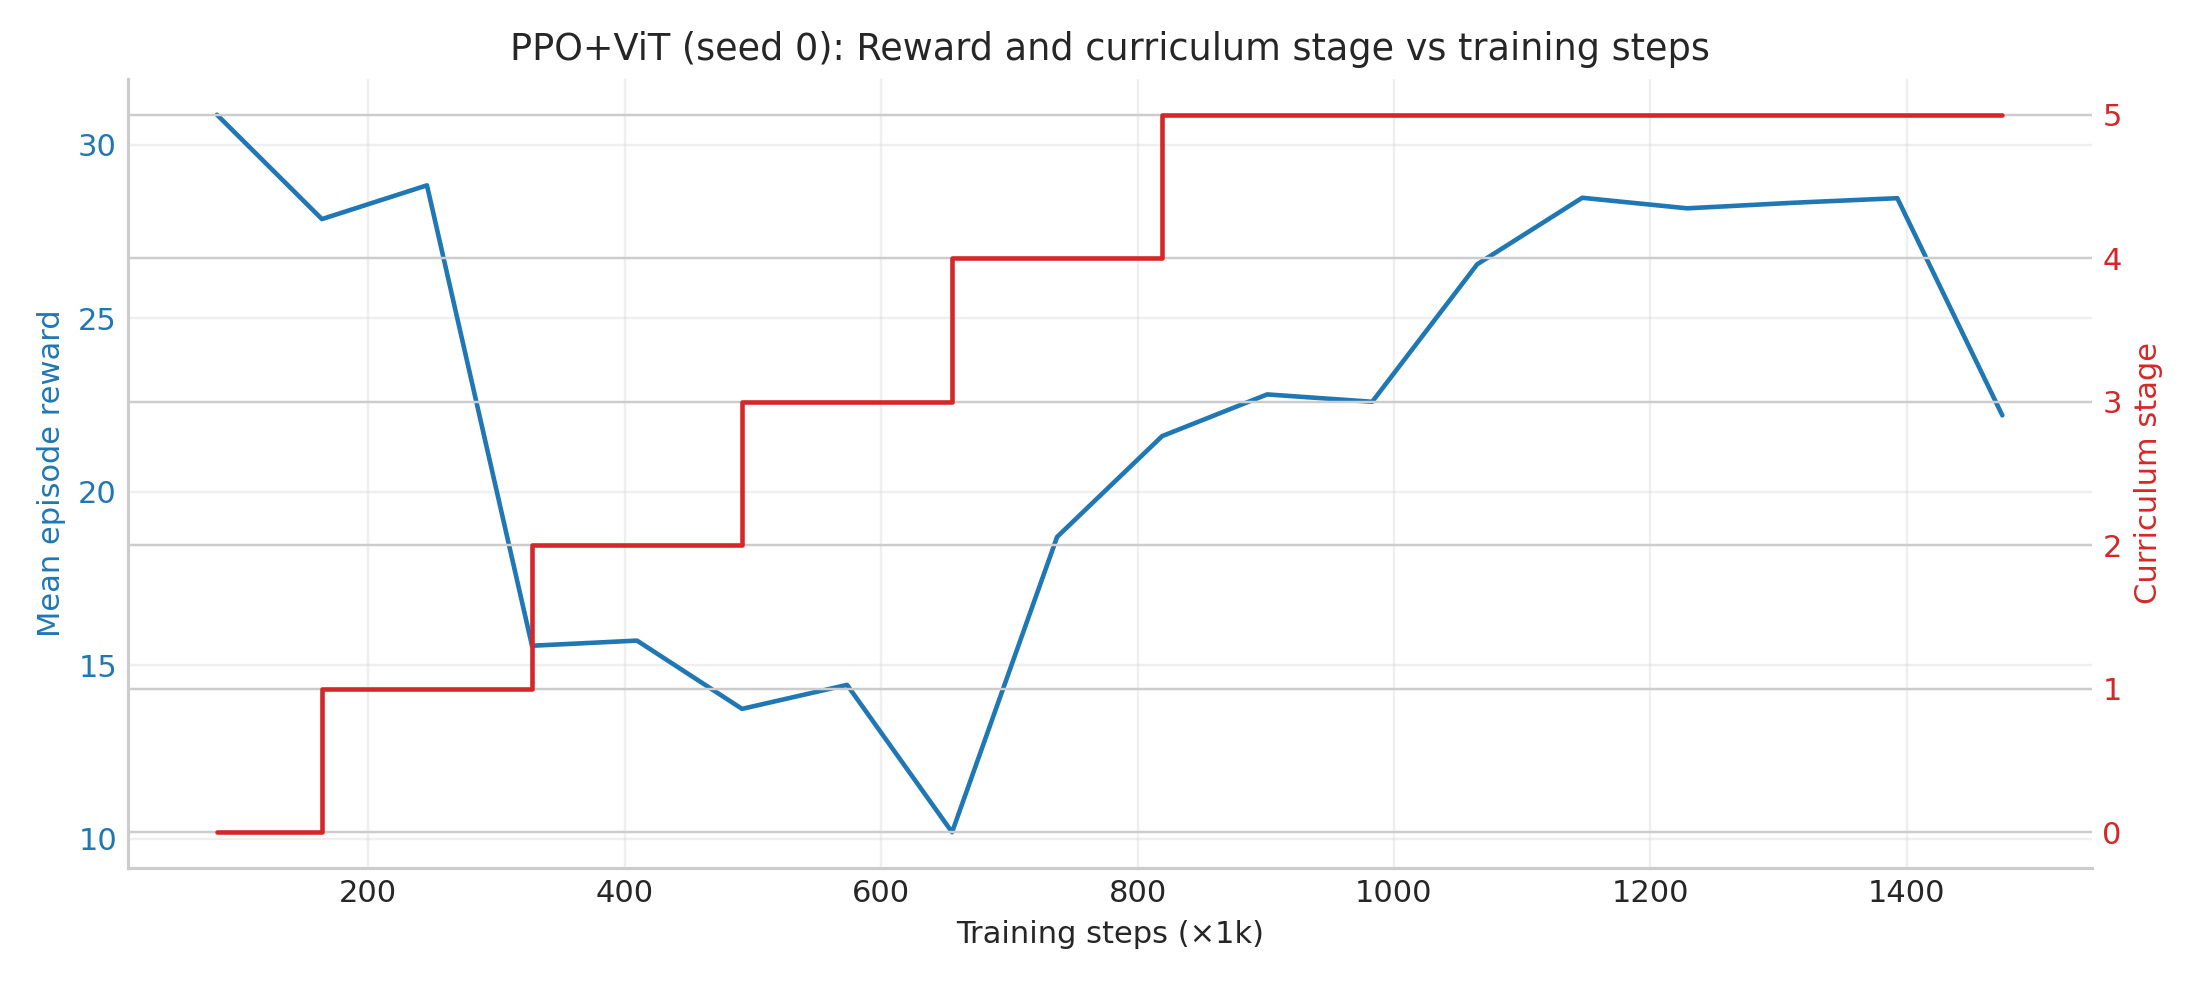
\includegraphics[width=\linewidth]{figures/fig_curriculum_progression.png}
\caption{Curriculum progression for the main PPO+ViT run.  The policy first
learns safe forward progress, then adapts to obstacles, moving obstacles,
wind, and sensor noise.}
\label{fig:curriculum}
\end{figure}

\begin{figure}[!t]
\centering
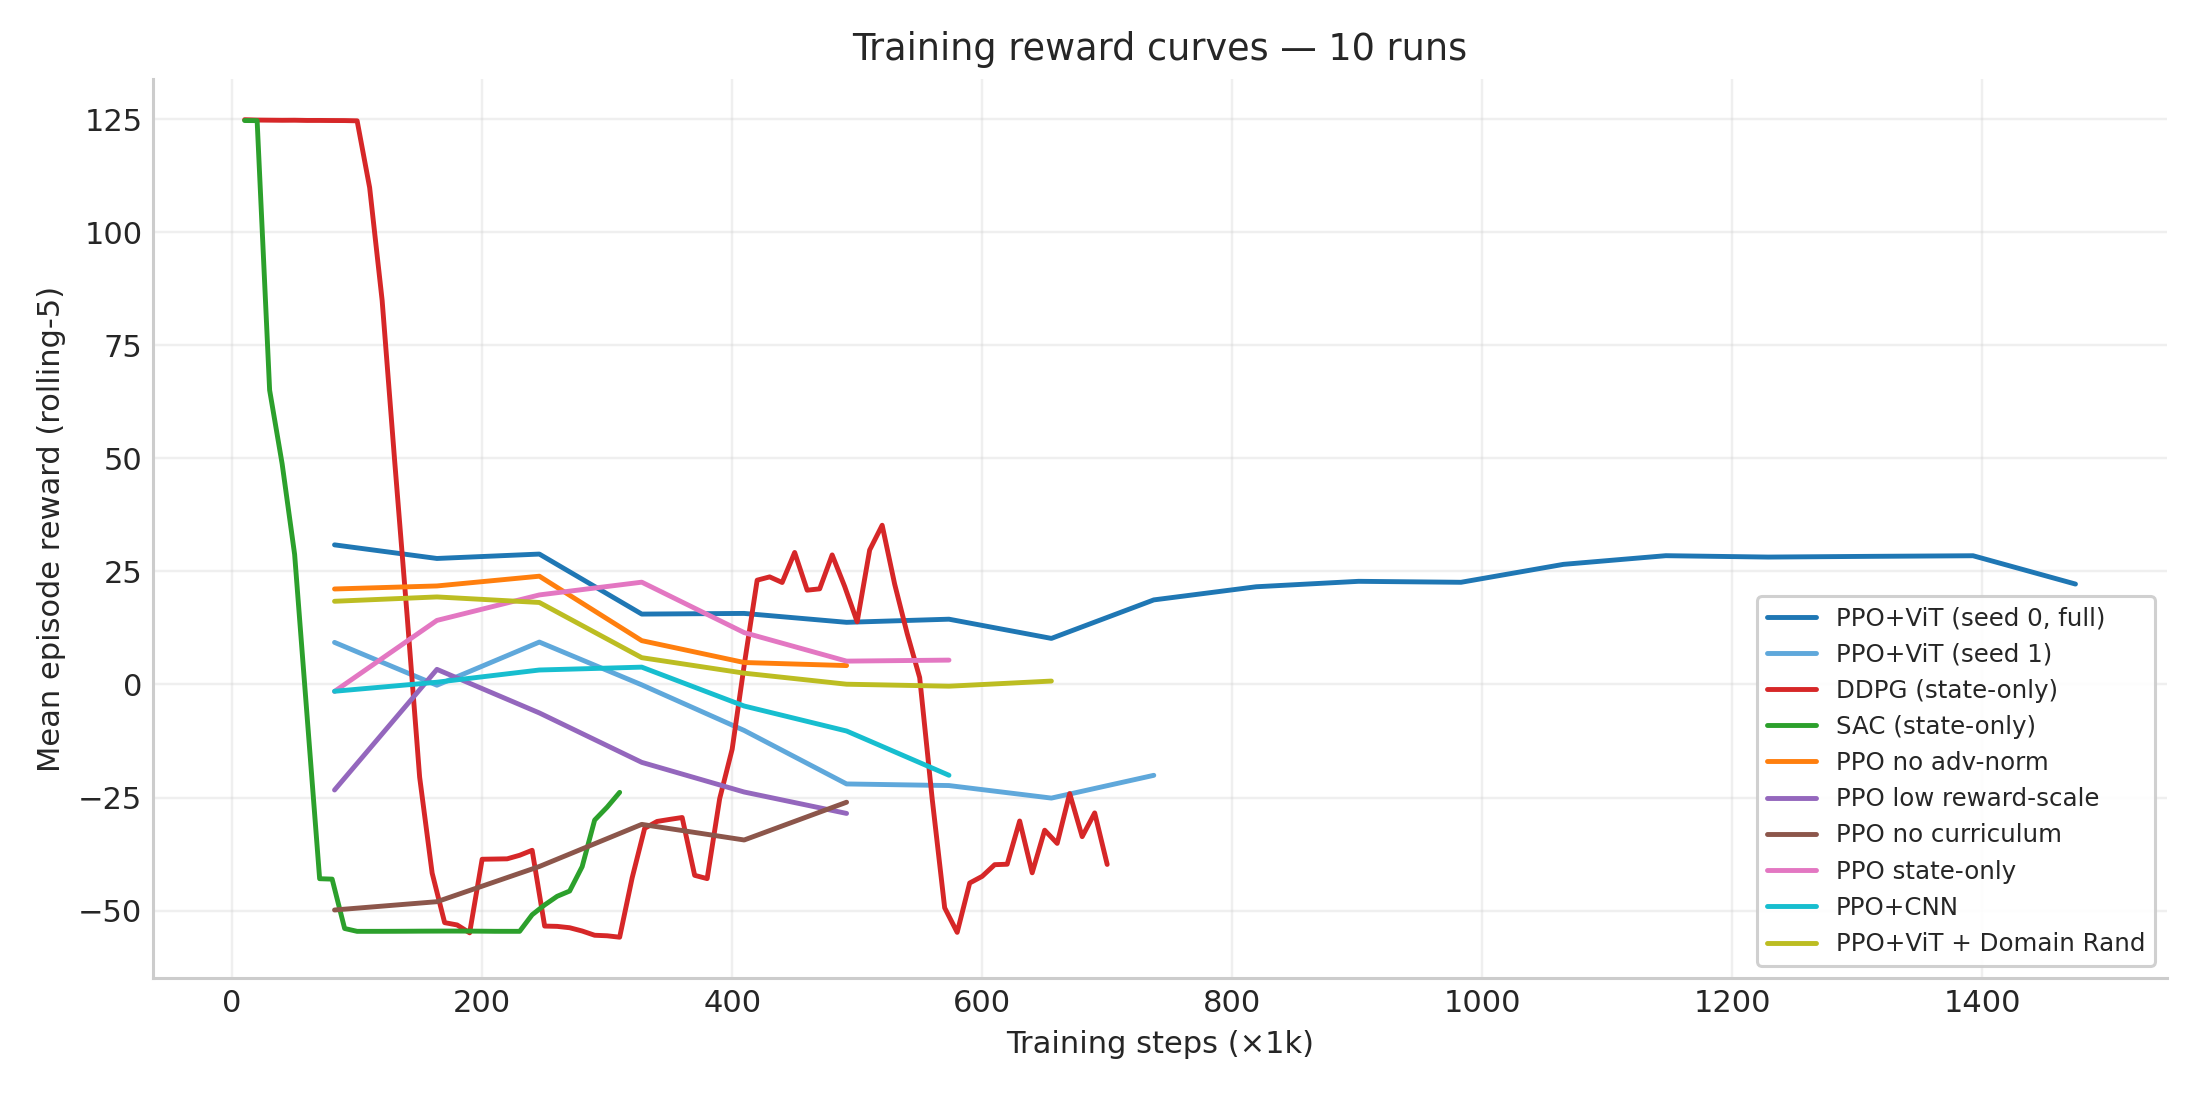
\includegraphics[width=\linewidth]{figures/fig_reward_curves.png}
\caption{Training reward curves across methods and ablations.  PPO variants
show stable reward growth; off-policy baselines collapse early under the
cluttered windy stage.}
\label{fig:rewards}
\end{figure}

% =====================================================================
\section{Results and Discussion}

\begin{table*}[!t]
\centering
\caption{Final-stage comparison using $N=30$ evaluation episodes.}
\label{tab:results}
\resizebox{0.96\textwidth}{!}{%
\begin{tabular}{@{}llrrrrrrr@{}}
\toprule
\headcell{Run} & \headcell{Algo} & \headcell{Seed} & \headcell{Steps}
& \headcell{Params} & \headcell{Success} & \headcell{Coll.}
& \headcell{Reward} & \headcell{Ep. len}\\
\midrule
PPO+ViT full              & ppo  & 0  & 1,507,328 & 1,002,311 & \textbf{1.000} & 0.000 & \textbf{124.85} & 150.6\\
PPO+ViT + Domain Rand.    & ppo  & 0  &   704,512 & 1,002,311 & 1.000 & 0.000 & 124.57 & 205.1\\
PPO no curriculum         & ppo  & 42 &   507,904 & 1,002,311 & 1.000 & 0.000 & 124.45 & 226.8\\
PPO+ViT seed 1            & ppo  & 1  &   802,816 & 1,002,311 & 1.000 & 0.000 & 124.33 & 279.6\\
PPO no adv-norm           & ppo  & 42 &   507,904 & 1,002,311 & 1.000 & 0.000 & 124.19 & 223.7\\
PPO state-only            & ppo  & 42 &   606,208 &    70,919 & 0.867 & 0.133 & 105.24 & 314.4\\
PPO low reward-scale      & ppo  & 42 &   507,904 & 1,002,311 & 1.000 & 0.000 &  28.90 & 1023.1\\
PPO+CNN                   & ppo  & 42 &   606,208 & 1,028,295 & 0.000 & 1.000 &  19.77 & 126.2\\
SAC state-only            & sac  & 0  &   300,000 &   213,256 & 0.000 & 1.000 & -42.16 & 12.3\\
DDPG state-only           & ddpg & 0  &   700,000 &   141,572 & 0.000 & 1.000 & -53.40 & 19.1\\
\bottomrule
\end{tabular}}
\end{table*}

\begin{figure*}[!t]
\centering
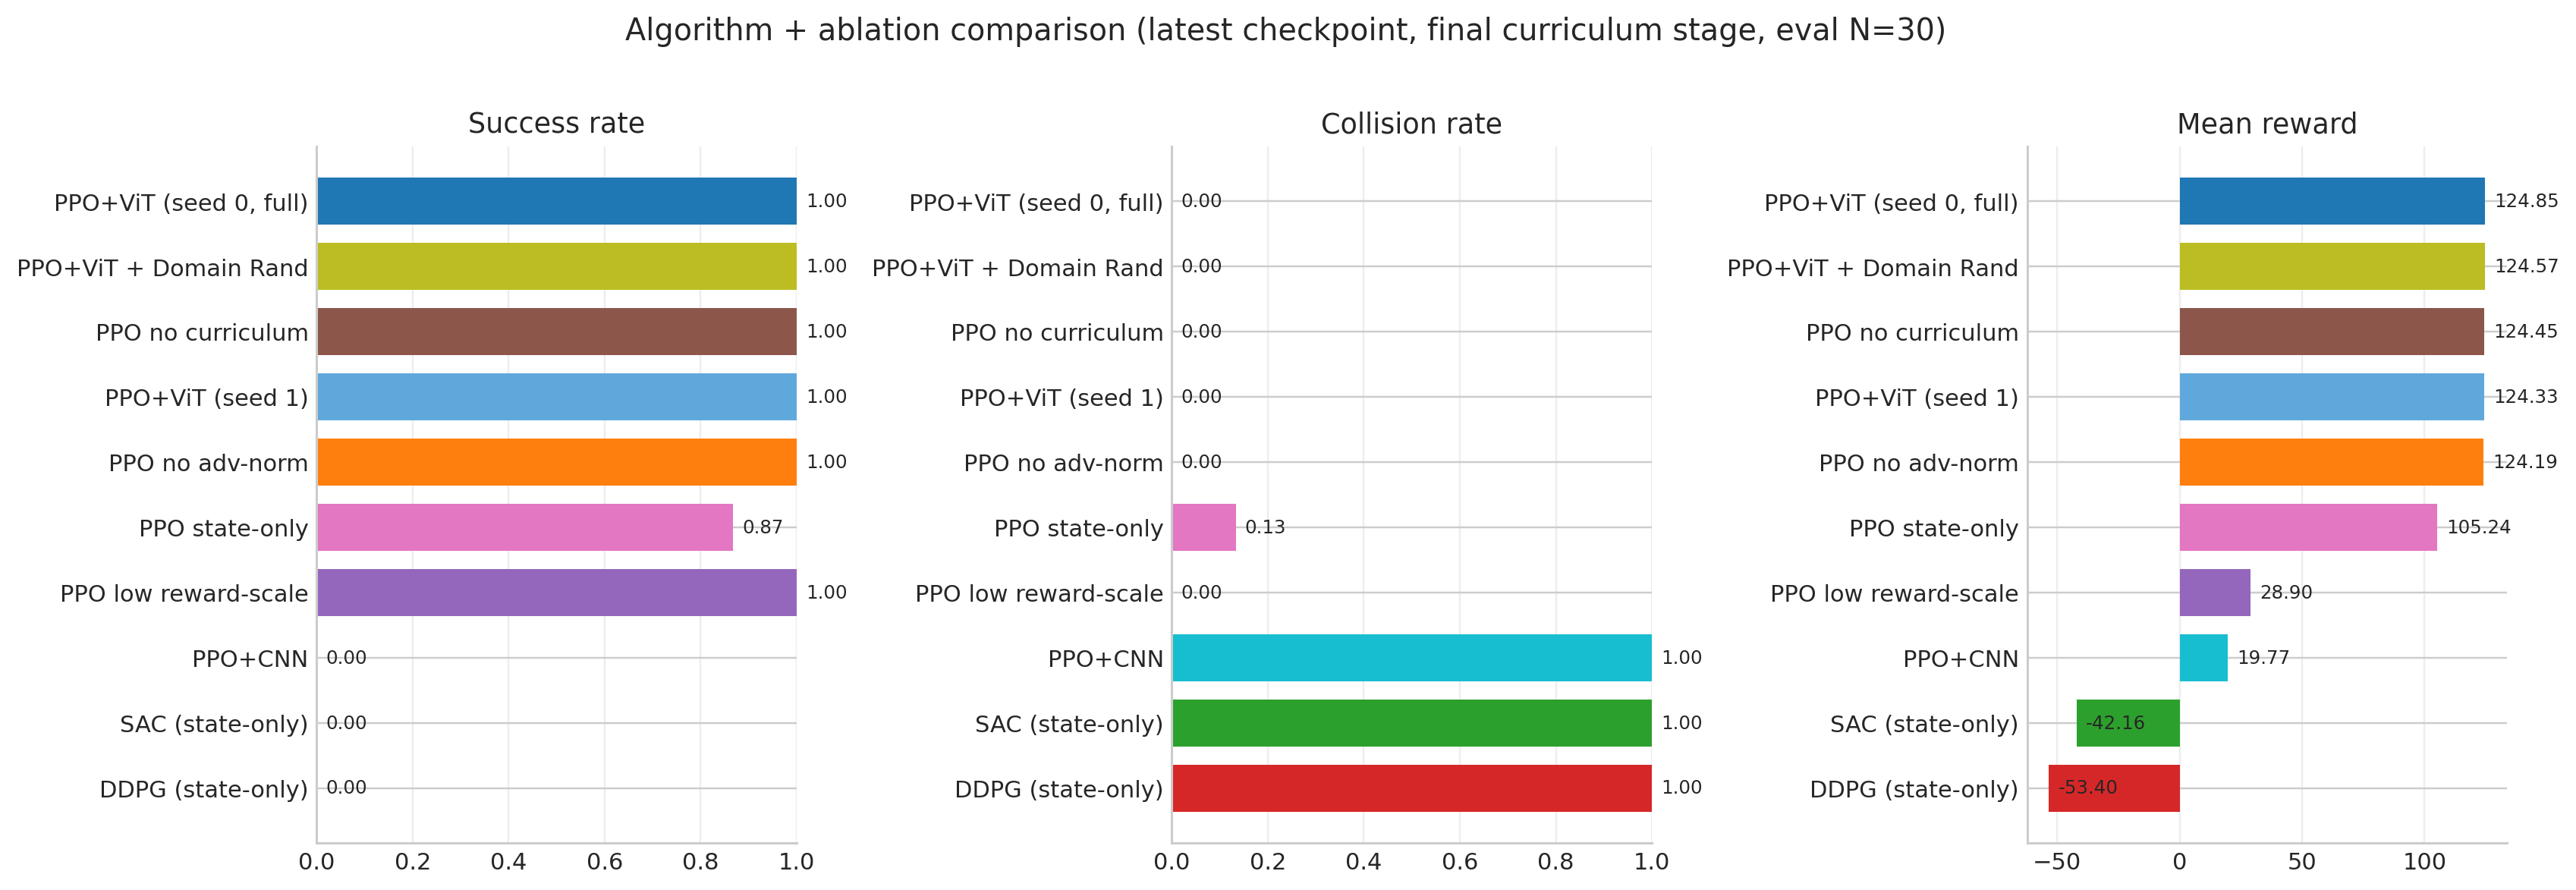
\includegraphics[width=0.95\textwidth]{figures/fig_comparison_bars.png}
\caption{Comparison across algorithms and ablations.  The contrast between
PPO+ViT and the off-policy baselines is strongest in collision rate and mean
return, not merely in final success labels.}
\label{fig:comparison}
\end{figure*}

\textbf{Why PPO performed best.}
PPO limits each policy update with a clipped objective, which is important
when a small visual-policy change can cause a collision.  It also learns from
fresh on-policy rollouts, avoiding the stale replay-distribution mismatch
that affected DDPG and SAC as the curriculum changed.

\textbf{Why DDPG and SAC collapsed.}
Both off-policy baselines rely on critic estimates.  In this environment,
small value errors are amplified because many actions lead quickly to
collision, and the replay buffer mixes samples from changing curriculum
stages.  DDPG also has brittle deterministic exploration; SAC explores more,
but still needs accurate Q-functions under high terminal penalties.  Their
short episode lengths and 100\% collision rates show failure before meaningful
goal-directed behavior emerges.

\textbf{Why vision helped.}
State-only PPO receives wall distances and forward clearance but lacks rich
spatial information about obstacle shape and visual layout.  It still learns
some navigation, but success drops to 86.7\% and variance increases.  The
ViT policy succeeds because attention over image patches helps encode the
global corridor opening and obstacle configuration.

\textbf{Why curriculum mattered.}
The no-curriculum ablation can eventually converge, but curriculum improves
training reliability: early wide-corridor stages provide non-collision
rollouts and meaningful progress rewards, then later stages introduce wind
and moving obstacles after basic goal-reaching has been learned.

% =====================================================================
\section{Generalization Analysis}

\begin{figure}[!t]
\centering
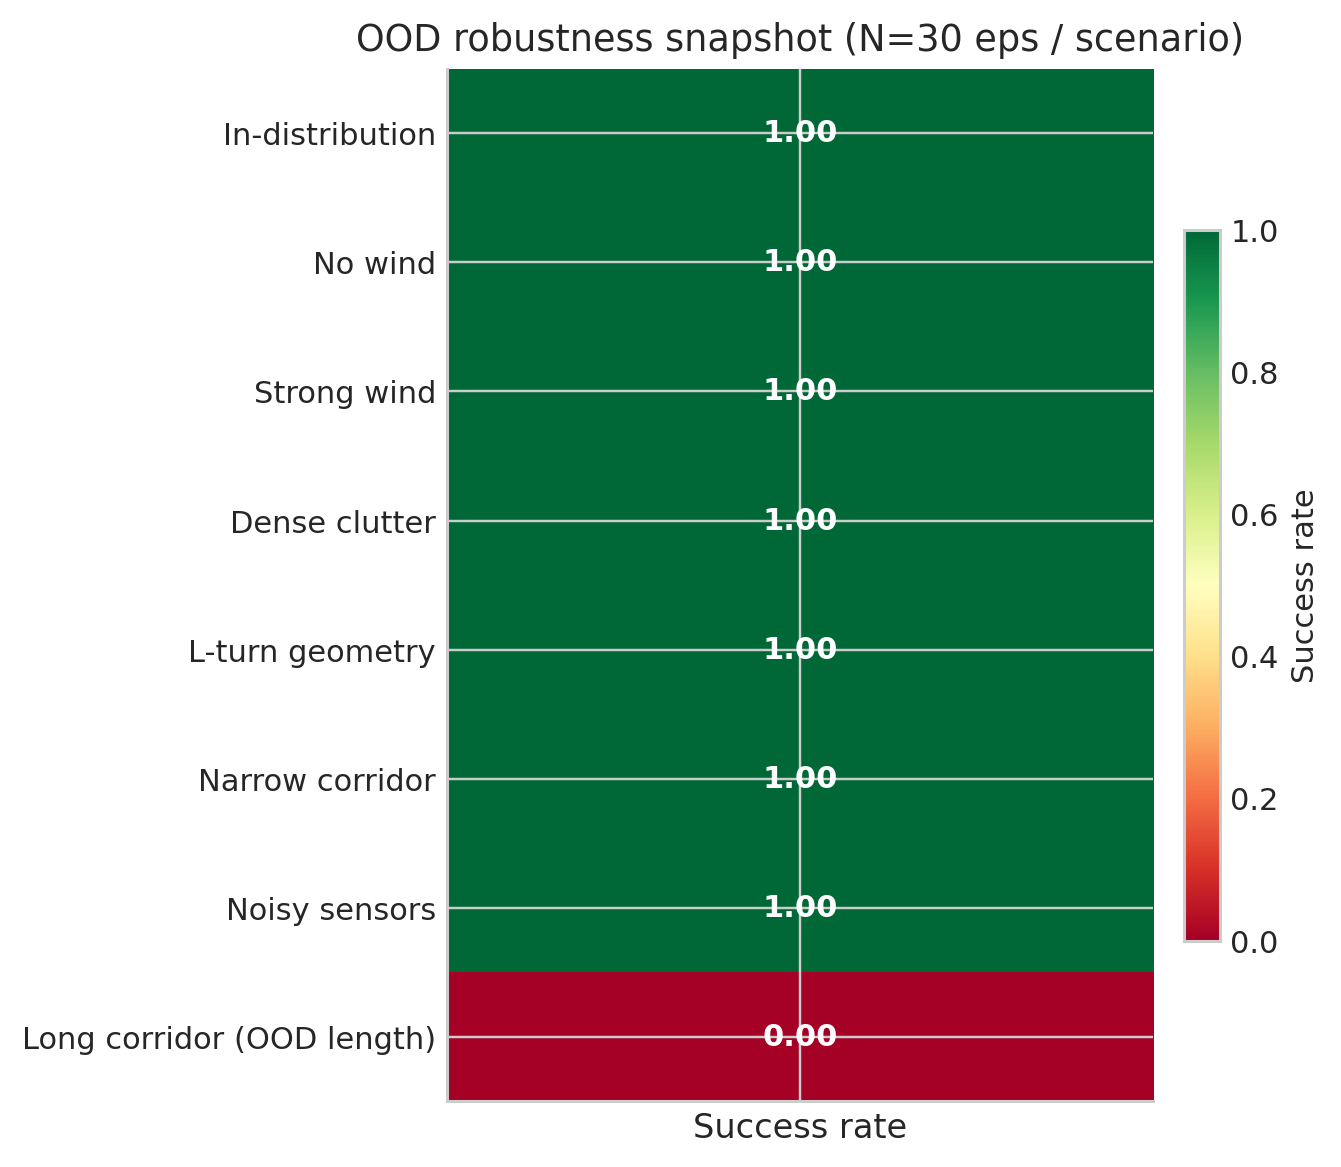
\includegraphics[width=\linewidth]{figures/fig_generalization_heatmap.png}
\caption{Success-rate heatmap for the frozen PPO+ViT checkpoint.  The policy
generalizes across most perturbations but fails outside the trained corridor
length.}
\label{fig:heatmap}
\end{figure}

\begin{table}[!t]
\centering
\caption{OOD generalization, $N=30$ episodes per scenario.}
\label{tab:gen}
\resizebox{\linewidth}{!}{%
\begin{tabular}{@{}lrrrr@{}}
\toprule
\headcell{Scenario} & \headcell{Succ.} & \headcell{Coll.} &
\headcell{Reward} & \headcell{Len.}\\
\midrule
in-distribution       & 1.00 & 0.00 & 124.76 & 150.5\\
no wind               & 1.00 & 0.00 & 124.63 & 150.2\\
strong wind           & 1.00 & 0.00 & 124.78 & 150.4\\
dense clutter         & 1.00 & 0.00 & 124.76 & 150.5\\
turns                 & 1.00 & 0.00 & 124.68 & 152.9\\
narrow corridor       & 1.00 & 0.00 & 124.59 & 157.8\\
noisy sensors         & 1.00 & 0.00 & 124.63 & 158.3\\
long corridor         & 0.00 & 1.00 &   5.49 & 116.3\\
\bottomrule
\end{tabular}}
\end{table}

\begin{figure}[!t]
\centering
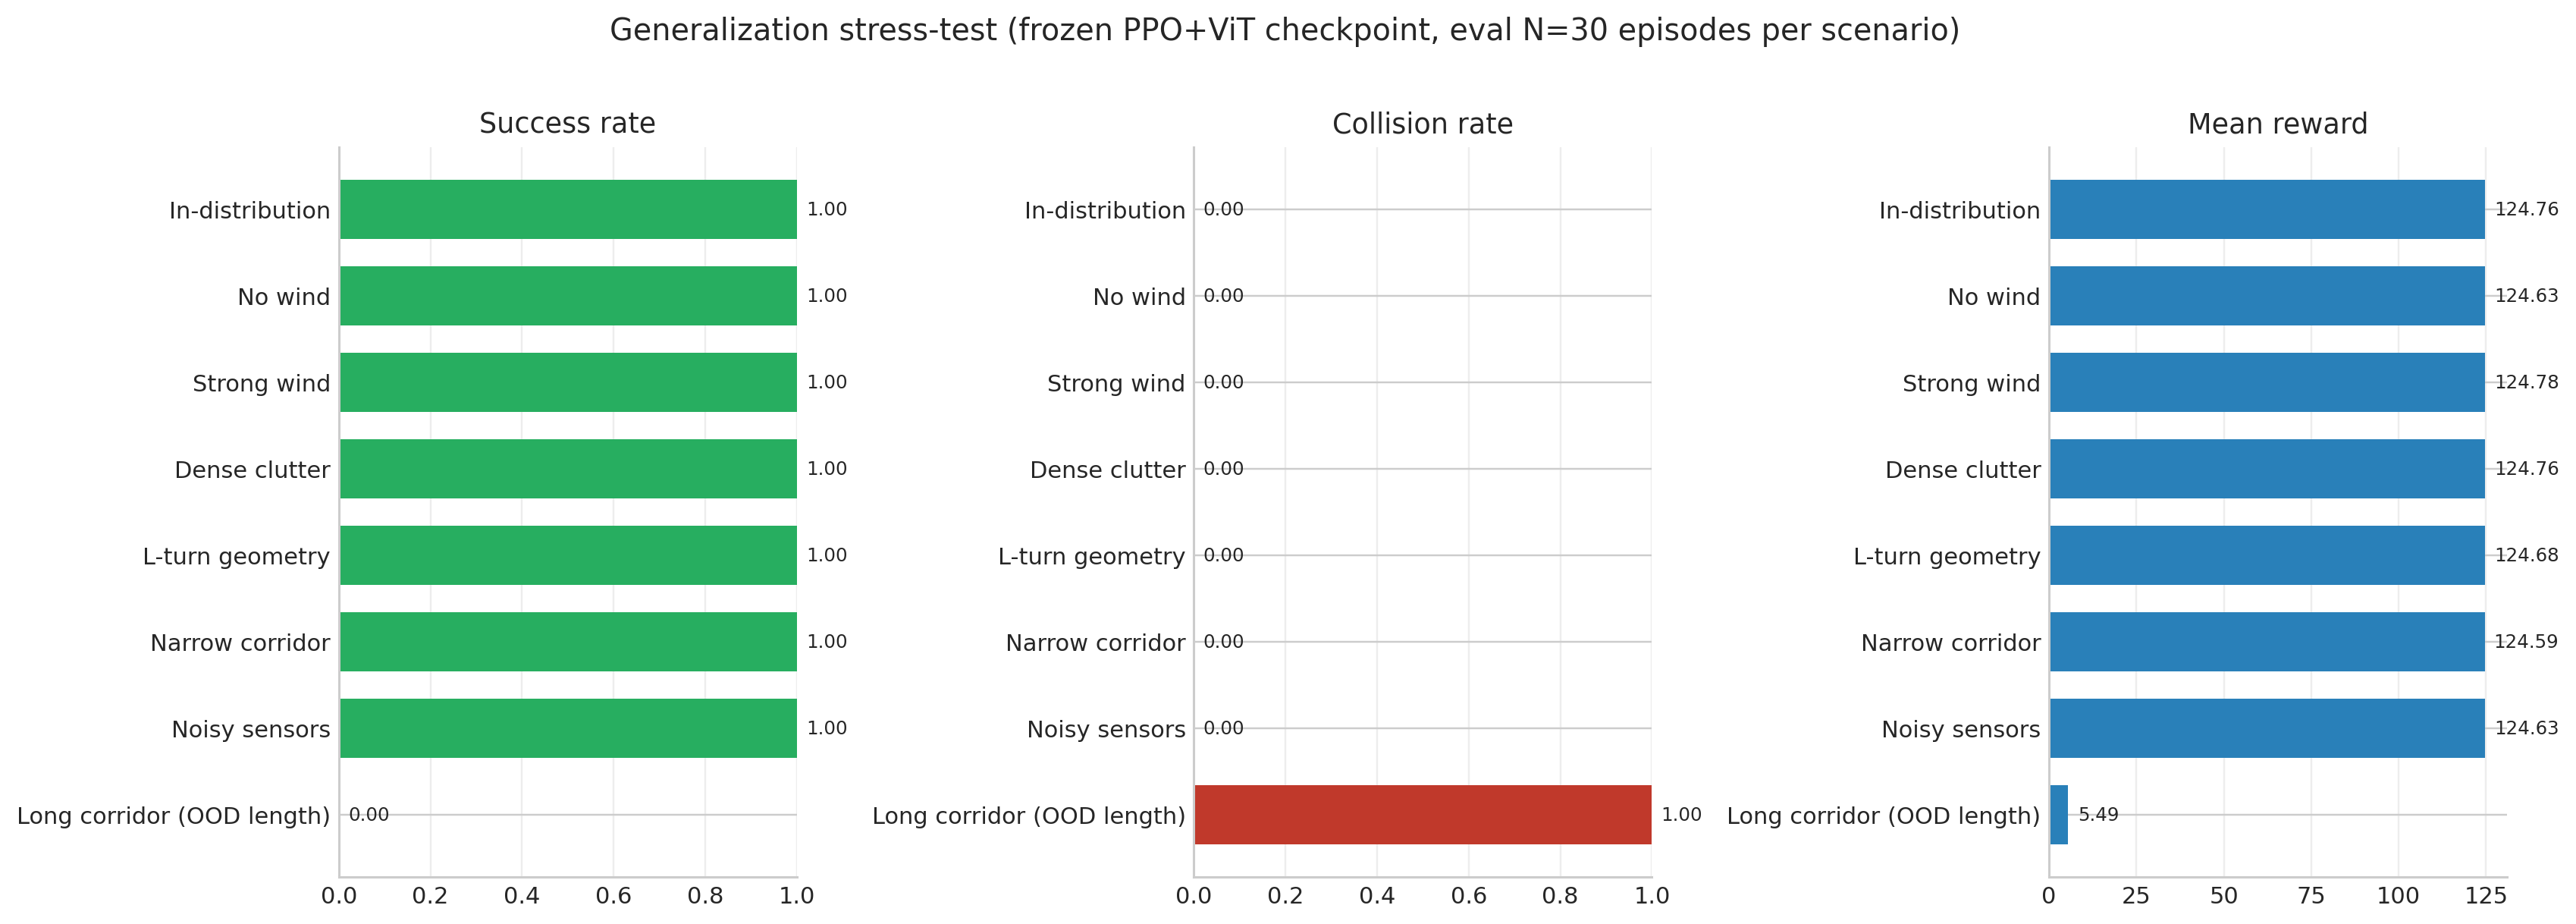
\includegraphics[width=\linewidth]{figures/fig_generalization.png}
\caption{Detailed OOD bars for success, collision, and reward.  Strong wind,
noise, and narrow corridors do not break the policy; length extrapolation
does.}
\label{fig:genbars}
\end{figure}

The generalization results are strong but informative.  The policy handles
wind intensity, sensor noise, clutter, and turns, which suggests it learned a
closed-loop navigation behavior rather than memorizing a single layout.
However, the 15 m long-corridor setting fails because the policy was trained
only on 10 m corridors.  This is a useful diagnosis: future curricula should
randomize corridor length, not only width, obstacle density, and wind.

% =====================================================================
\section{Conclusion}

This project demonstrates a complete RL pipeline for vision-based continuous
drone navigation.  The final PPO+ViT policy solves the full windy corridor
task with 100\% success and 0\% collision in final-stage evaluation, while
DDPG and SAC fail under the same environment.  The ablations show that the
result is not just a final-score artifact: reward scale affects efficiency,
vision improves reliability, the ViT encoder is substantially stronger than
the CNN variant in this setting, and domain randomization preserves
performance while preparing for sim-to-real transfer.  The project therefore
satisfies the core RL expectations: real-world motivation, formal
MDP/POMDP definition, multiple RL methods, principled reward shaping,
curriculum learning, and analytical comparison.

% =====================================================================
\section{Limitations and Future Work}

\textbf{Limitations.}
First, the simulator is PyBullet rather than Flightmare/Isaac, so image
realism is limited even though dynamics and collision contacts are modeled.
Second, the policy is not deployed on a physical drone; real hardware would
introduce latency, camera calibration, actuator limits, and safety constraints.
Third, only two PPO seeds and one seed per ablation were feasible on the
available GPU.  Fourth, the long-corridor failure shows limited extrapolation
outside the training geometry.

\textbf{Future work.}
The most direct improvements are: (i) randomize corridor length, textures,
lighting, mass, damping, wind correlation, and control latency; (ii) test
recurrent policies (GRU/LSTM) for longer-horizon wind effects; (iii) improve
exploration for off-policy baselines using TD3/SAC with visual encoders and
targeted replay; (iv) use stronger transformer backbones or hybrid CNN-ViT
encoders; (v) study multi-agent RL for dynamic obstacle negotiation; and
(vi) transfer to a small real drone using domain randomization and a safety
filter.

% =====================================================================
\section{GitHub Repository Link}

The full codebase, configs, runs, and report assets are available at:
\begin{center}
\small \repo
\end{center}
The demo video used for qualitative inspection is available at:
\begin{center}
\small \demolink
\end{center}

\begin{tcolorbox}[enhanced, breakable,
  colback=boxBg, colframe=cGray!55, boxrule=0.4pt, arc=2pt,
  left=5pt, right=5pt, top=3pt, bottom=3pt,
  title=\footnotesize\textbf{Reproducibility commands},
  fonttitle=\footnotesize, coltitle=black,
  colbacktitle=cGray!18, attach boxed title to top left={xshift=4pt,yshift=-2pt},
  boxed title style={colframe=cGray!55, boxrule=0.3pt, arc=1pt}]
\begin{lstlisting}[basicstyle=\ttfamily\scriptsize,breaklines=true,
  columns=fullflexible,keepspaces=true]
./scripts/run_queue.sh
python scripts/aggregate_all.py --episodes 30
python scripts/eval_generalization.py \
  --checkpoint runs/best_vit/ppo_seed0_t1p5m/checkpoints/checkpoint_1507328.pt \
  --config drone_rl/configs/ppo_best.yaml \
  --episodes 30 --out report_artifacts/generalization.csv
python scripts/figures/make_figures.py
\end{lstlisting}
\end{tcolorbox}

% =====================================================================
\begin{thebibliography}{9}
\small

\bibitem{schulman2017ppo}
J. Schulman, F. Wolski, P. Dhariwal, A. Radford, and O. Klimov.
\newblock Proximal Policy Optimization Algorithms.
\newblock arXiv:1707.06347, 2017.

\bibitem{lillicrap2015ddpg}
T. Lillicrap et al.
\newblock Continuous Control with Deep Reinforcement Learning.
\newblock arXiv:1509.02971, 2015.

\bibitem{haarnoja2018sac}
T. Haarnoja, A. Zhou, P. Abbeel, and S. Levine.
\newblock Soft Actor-Critic: Off-Policy Maximum Entropy Deep Reinforcement
Learning with a Stochastic Actor.
\newblock ICML, 2018.

\bibitem{dosovitskiy2020vit}
A. Dosovitskiy et al.
\newblock An Image is Worth 16x16 Words: Transformers for Image Recognition
at Scale.
\newblock ICLR, 2021.

\bibitem{bengio2009curriculum}
Y. Bengio, J. Louradour, R. Collobert, and J. Weston.
\newblock Curriculum Learning.
\newblock ICML, 2009.

\end{thebibliography}

\end{document}
